\section{Введение} 

\subsection{Ограниченная эллиптическая задача трех тел и пояс астероидов}
В настоящей работе рассматривается плоская ограниченная эллиптическая задача трех тел в случае резонансного отношения периодов 3:1 малого тела и Юпитера. Данная задача является предельным вариантом общей задачи трех тел, исследованию которой посвящено большое число работ. Начиная с исследований Ньютона, Эйлера, Клеро, Даламбера, Лапласа, Лагранжа, Якоби, Коши, Пуанкаре, задача трех тел дала развитие не только анализу, но и многим другим разделам математатики. 

Рассмотрим движение трех тел с гравитационным взаимодействием в пространстве. Будем обозначать величины, связанные с различными телами, индексами $A,J,S$ (условно астероид, Юпитер, Солнце). Тогда уравнения движения принимают вид:
\begin{equation*}
 \begin{cases}
   m_S \v{\ddot{r_S}} = 
   \frac{G m_S m_J}{|\v{r_J-r_S}|^3} (\v{r_J-r_S})+
   \frac{G m_S m_A}{|\v{r_A-r_S}|^3} (\v{r_A-r_S}), 
   \\
   m_J \v{\ddot{r_J}} = 
   \frac{G m_J m_S}{|\v{r_S-r_J}|^3} (\v{r_S-r_J})+
   \frac{G m_J m_A}{|\v{r_A-r_J}|^3} (\v{r_A-r_J}),
   \\
   m_A \v{\ddot{r_A}} = 
   \frac{G m_A m_S}{|\v{r_S-r_A}|^3} (\v{r_S-r_A})+
   \frac{G m_A m_J}{|\v{r_J-r_A}|^3} (\v{r_J-r_A}),
 \end{cases}
\end{equation*}
где $m_{k}$ ($k\in \{A, J, S\}$) - масса $k$-го тела, $r_{k}$ - его радиус-вектор, $G$ - гравитационная постоянная. Поделив уравнения на массы, стоящие в левых частях равенств, можно заметить, что уравнения не теряют смысл и в пределе, когда одна или несколько масс обращаются в нуль.

Данная система является динамической системой с 9 степенями свободы. Однако, если предположить, что движение всех тел происходит в плоскости, то число степеней свободы системы уменьшается до 6, что заметно упрощает дальнейший анализ. При этом задача называется плоской задачей трех тел. Такое предположение является физически обоснованным, поскольку большое число наблюдаемых звездных систем могут считаться плоскими в том смысле, что один из их линейных рамеров много меньше двух других. Кроме того, из астрономических наблюдений известно, что, если астероид влетает в солнечную систему под большим углом, то он не задерживается в ней надолго.

Предположим, что массы тел удовлетворяют соотношению: 
$$m_A \ll m_J \ll m_S.$$ 

В таком случае, учитывая малость $m_A$, слагаемые, содержащие его в правой части, можно отбросить:
\begin{equation*}
 \begin{cases}
   \v{\ddot{r}_{S}} = 
   \frac{G m_J}{|\v{r_J-r_S}|^3} (\v{r_J-r_S}),
   \\
   \v{\ddot{r}_{J}} = 
   \frac{G m_S}{|\v{r_S-r_J}|^3} (\v{r_S-r_J}),
   \\
   \v{\ddot{r}_{A}} = 
   \frac{G m_S}{|\v{r_S-r_A}|^3} (\v{r_S-r_A})+
   \frac{G m_J}{|\v{r_J-r_A}|^3} (\v{r_J-r_A}).
 \end{cases}
\end{equation*}

Заметим, что первые два уравнения не зависят от характеристик астероида и, таким образом, описывают задачу Кеплера о движении двух тел под действием гравитационных сил. Как известно \cite{dub}, задача Кеплера интегрируема. С другой стороны, третье уравнение описывает движение астероида в гравитационном поле двух массивных тел. Такая задача называется ограниченной плоской задачей трех тел.

Перейдем в систему координат Якоби \cite{dub}, связанную с центром масс тел $S$ и $J$:
$$
\v{r} = \v{r_J}-\v{r_S},\quad
\v{\rho} = \frac{m_S}{m_J+m_S} \v{r} - \v{r_J} + \v{r_A},\quad
\v{r_c} = \v{r_J} - \frac{m_S}{m_J+m_S} \v{r}.
$$

Производя замену переменных и учитывая слагаемые, возникающие при переходе в неинерциальную систему отсчета, получаем:
\begin{equation*}
\begin{cases}
\v{\ddot{r_c}} = 0, \\
\v{\ddot{r}} = -\frac{G(m_S+m_J)}{r^3} \v{r},  \\
\v{\ddot{\rho}} = [\v{\rho} \times \frac{d \dot{\Omega}}{dt}]  + 2[\v{\dot{\rho}} \times \v{\Omega}] + [\v{\Omega} \times [\v{\rho} \times \v{\Omega}]] + \frac{1}{m_A} \frac{G m_A m_S}{|\v{r_S-r_A}|^3} (\v{r_S-r_A})+
   \frac{G m_A m_J}{|\v{r_J-r_A}|^3} (\v{r_J-r_A}),  
 \end{cases}
\end{equation*}
где
$$
\v{\Omega} = \frac{[\v{r_c} \times \v{\dot{r_c}}]}{r_c^2}.
$$

Масштабным преобразованием координат и переобозначением констант можно  добиться того, что параметры системы удовлетворяют следующим условиям:
$$
G = 1,\quad 
m_j = \mu,\quad 
m_s = 1 - \mu,\quad
|\v{\Omega}| = 1.
$$

Тогда уравнения движения, описывающие движение малого тела, имеют вид:
\begin{equation*}
 \begin{cases}
   \ddot{\rho_x}=+2 \dot{\rho_y} + \rho_x - \frac{\partial U}{\partial \rho_x}, \\
   \ddot{\rho_y}=-2 \dot{\rho_x} + \rho_y - \frac{\partial U}{\partial \rho_y},
 \end{cases}
\end{equation*}
$$U(r, \v{\rho}) = - \frac{1-\mu}{\sqrt{\big(\rho_x + \mu r \big)^2 + \rho_y^2}} - \frac{\mu}{\sqrt{\big(\rho_x - (1-  \mu ) r \big)^2 + \rho_y^2}}.$$
Полученная система уравнений является системой Лагранжа с лагранжианом:
$$L = \frac{\dot{\rho_x}^2 + \dot{\rho_y}^2}{2} + \frac{{\rho_x}^2 + {\rho_y}^2}{2} + \rho_x \dot{\rho_y} - \rho_y \dot{\rho_x} - U(r,\v{\rho}) .$$
Применяя к лагранжиану преобразование Лежандра и вводя переменные:
$$
x = \rho_x,\quad
y = \rho_y,\quad
p_x = \dot{x} - y,\quad
p_y = \dot{y} + x,
$$
получаем гамильтониан системы:
$$H = \frac{p_x^2 + p_y^2}{2} + p_xy - p_yx + U(r,\v{\rho}).$$

Потенциал в гамильтониане содержит параметр $r = |\v{r}|$ (расстояние между Солнцем и Юпитером), который определяется из уравнения:
$$\v{\ddot{r}} = -\frac{G(m_S+m_J)}{r^3} \v{r},$$
и в общем случае зависит от времени. Это уравнение является частным случаем задачи Кеплера, для которой известно точное решение. 

Известно, что эксцентриситет Юпитера достаточно мал (порядка $e_{J}\approx 0.05$), и потому его орбита близка к круговой. В пределе $e_{J}\to 0$ расстояние $r$ постоянно и мы получаем так называемую круговую плоскую ограниченную задачу трех тел. Данная задача описывается системой с двумя степенями свободы. Следует отметить, что круговая задача интегрируема, т.к. помимо интеграла энергии, она имеет второй интеграл движения - интеграл Якоби:
$$
\dot \rho_{x}^{2} + \dot \rho_{y}^{2} - \rho_{x}^{2} - \rho_{y}^{2} - 2 U(\rho_{x}, \rho_{y}) = {\rm const}.
$$

Однако, как показывают исследования \cite{fejoz, kaloshin}, учет эксцентриситета Юпитера $e_J$ является необходимым для рассмотрения хаотических процессов в системе. В предположении $e_{J}>0$ задача называется плоской эллиптической ограниченной задачей трех тел.



















































\subsection{Окрестность резонанса}
Для рассмотрения резонансного случая удобно перейти в систему координат Делоне, в которой гамильтониан имеет вид \cite{plummer}:
$$H = - \frac{(1-\mu)^2}{2L^2} - \mu R(L, \rho_1, \rho_2, l, \omega_1, \omega_2),$$
где возмущающая функция $R$ равна:
$$R = \sum_{s-j-k+p-m-n=0, s \geq 0} K^{sjkpmn}(L, \rho_1, \rho_2) \cos(s l + p l_J + j \omega_1 + k \omega_2 + m \omega_{1J} + n \omega_{2J}).$$
Здесь $(1-\mu)$ - масса Солнца, $\mu \approx \frac{1}{1000}$ - масса Юпитера, являющаяся малым параметром. Все углы, относящиеся к Юпитеру, обозначены индексом $J$, а углы, связанные с астероидом, обозначаются без индекса, гравитационная постоянная полагается равной единице. В терминах эллиптических элементов переменные выражаются формулами:
$$L = \sqrt{(1-\mu)a},$$
$$\rho_1 = \sqrt{(1-\mu)a}(1-\sqrt{1-e^2}),$$
$$\rho_2 = \sqrt{(1-\mu)a(1-e^2)}(1-\cos i),$$
здесь $a$ - большая полуось, $e$ - эксцентриситет, $i$ - наклон орбиты, $l$ - средняя долгота, $\omega_1$ - долгота перицентра, $\omega_2$ - долгота восходящего узла.

\begin{figure}[htp]
\centering
\includegraphics[scale=0.12]{img/Orbit1-mean.png}
\caption{Средняя долгота $l = \omega_1 + \omega_2 + M$, где $M$ - средняя аномалия}
\end{figure}

Резонанс возникает когда аргументы косинусов близки к стационарным \cite{wis2}:
$$s l + p l_J + j \omega_1 + k \omega_2 + m \omega_{1J} + n \omega_{2J} = \text{const}.$$

Учитывая, что средняя долгота $l$ меняется значительно быстрее остальных углов, получаем резонансное условие (точка обозначает производную по времени):
$$s \dot l + p \dot l_J \approx 0, $$
которое можно переписать в виде:
$$\dot l \approx \frac{-p}{s} \dot l_J \equiv \frac{s+q}{s} \dot l_J.$$

Число $q$ называется порядком резонанса и для исследуемого в данной работе резонанса 3:1 $q=2$, $s=1$.

Учтем, что рассматривается плоская задача, следовательно, $i=0$, $\rho_2=0$, $\omega_2=0$. Подставляя известные коэфициенты ряда и отбрасывая все члены старше второго порядка по $e_J$, получаем \cite{wis2}:
$$H = - \frac{(1-\mu)^2}{2L^2} - \mu R_{sec}(\rho_1, \omega_1) - \mu R_{res}(L,l,\rho_1,\omega_1),$$
где $R_{sec}(\rho_1, \omega_1) = - 2 \rho_1 F - e_J G \sqrt{2 \rho_1} \cos \omega_1$ - секулярная часть возмущающей функции, содержащая медленно меняющиеся со временем члены и в общем случае не периодические, 

$R_{res}(L,l,\rho_1,\omega_1) = 2 \rho_1 C \cos(l-\omega_1-3 l_J)+e_J^2E \cos(l - 3 l_J)$ - резонансная часть возмущающей функции, содержащая медленно изменяющиеся периодические члены.

Масштабным преобразованием можно добиться  \cite{wis2}:
$$a_J=1, \dot l_J= 1 .$$

Производя замену:
$$\Lambda = L - L_{res},$$
$$\lambda = l - 3 l_J,$$
$$x = \sqrt{2 \rho_1} \cos \omega_1,$$
$$y = \sqrt{2 \rho_1} \sin \omega_1,$$
и раскладывая гамильтониан по степеням $\Lambda$, получаем в старшем порядке:
\begin{equation}
\label{Ham_res}
H = \alpha \frac{\Lambda^2}{2} + \mu \left( C(x^2-y^2)+e_J D x + e_J^2 E \right) \cos \lambda + \mu (2Cxy+e_J D y) \sin \lambda + \mu e_J G x + \mu F(x^2+y^2),
\end{equation}
где $L_{res} = \left( \frac{(1-\mu)^2}{3} \right)^\frac13$ - центр резонанса, определяемый условием резонансности 
$$
\dot \lambda = \frac{\partial H}{\partial L}|_{L=L_{res}}=0,$$
a постоянная $\alpha$: 
$$\alpha = -\frac{3(1-\mu)^2}{L_{res}^4} < 0.$$

Следует отметить, что $y$ и $\lambda$ являются координатами, а $x$ и $L$ сопряженными к ним импульсами. При этом фазовое пространство рассматриваемой системы  четырехмерно и, учитывая периодичность правой части уравнений по $\lambda$, можно считать, что:
$$(x,y,\Lambda,\lambda) \in \mathbb{R}^3 \times S^1 .$$

Коэфициенты $F,G,C,D,E,e_J$ являются известными константами, значения которых в случае системы Солнце-Юпитер можно найти, например, в \cite{wis1}.

Систему, описываемую гамильтонианом (\ref{Ham_res}), принято называть плоской эллиптической ограниченной задачей трех тел в случае главного резонанса 3:1.













































%%%%%%%%%%%%%%%%%%%%%%%%%%%%%%%%%%%%%%%%%%%%%%%%%%%%%%%%%%%%%%%%%%%
\subsection{Практические применения и классичский метод исследования}

Одним из возможных применений описанной выше задачи является исследование причин возникновения щелей Кирквуда -- определенных областей в поясе астероидов между орбитами Юпитера и Марса, в которых траектории астероидов не могут находиться долгое время. Впервые данные промежутки были обнаружены в 1866 году Д. Кирквудом. Согласно наблюдениям, щели соответствуют целочисленным отношениям периодов орбит астероидов к периоду обращения Юпитера вокруг Солнца. Наиболее отчетливо различимы щели с отношениями: 2:1, 3:1, 5:2, 7:3. 

\begin{figure}[H]
\centering
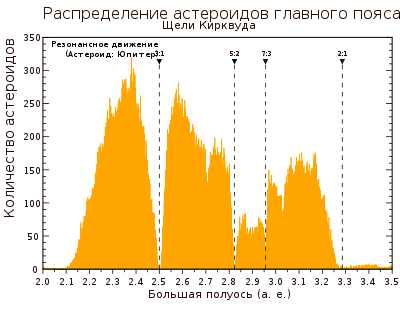
\includegraphics[scale=0.6]{img/gaps.png}
%\caption{Щели Кирквуда \cite{graph}}
\caption{Щели Кирквуда}

\end{figure}

\begin{figure}[H]
\centering
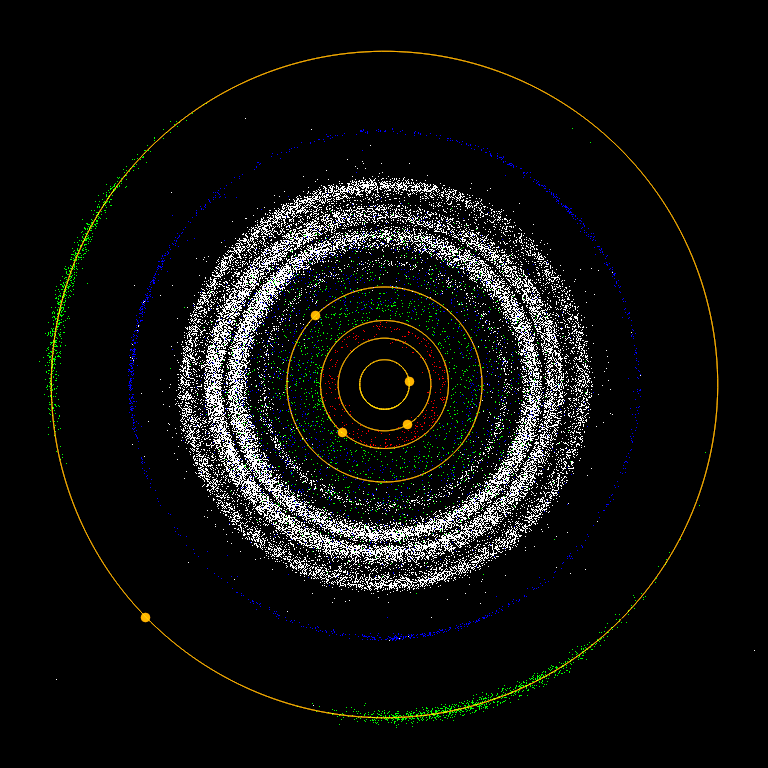
\includegraphics[scale=0.25]{img/gaps2.png}
%\caption{Астероиды в Солнечной системе \cite{plot}}
\caption{Астероиды в Солнечной системе} 

\end{figure}

Большой вклад в исследование данного вопроса внес Д. Висдом, предложивший использовать метод усреднения для объяснения данного эффекта. Рассмотрим канонические уравнения для описанного выше гамильтониана \cite{wis1}:
\begin{equation}
    \begin{cases}
        \frac{d \Lambda}{dt} = \mu \big( u(x,y) \sin \lambda - v(x,y) \cos \lambda \big), \\
        \frac{d \lambda}{dt} = \alpha \Lambda,\\
        \frac{dx}{dt} = -\mu \left(2Fy+\frac{\partial u(x,y)}{\partial y} \cos \lambda + \frac{\partial v(x,y)}{\partial y} \sin \lambda \right), \\
        \frac{dy}{dt} = \mu \left( 2Fx+e_JG +\frac{\partial u(x,y)}{\partial x} \cos \lambda + \frac{\partial v(x,y)}{\partial x} \sin \lambda \right),
    \end{cases}
    \label{sys2}
\end{equation}
где введены обозначения
$$u(x,y) = C(x^2-y^2)+e_J Dx +e_J^2E,$$
$$v(x,y) = 2Cxy+e_JDy.$$

Так как $\frac{dx}{dt}$ и $\frac{dy}{dt}$ пропорциональны $\mu$, то характерное время изменения переменных $x$ и $y$ имеет порядок $\mu^{-1}$, что заметно больше времени малоамплитудных колебаний $\lambda$ (их характерное время порядка $\mu^{-\frac12}$). В силу этого, $x$ и $y$ можно разделить в сумму длинно- и короткопериодных частей: $x=\overline x + \xi$, $y=\overline y + \eta$, причем длиннопериодная часть описывается усредненной системой уравнений:
\begin{equation}
    \begin{cases}
        \frac{d \overline x}{dt} = -\mu \left( 2F \overline y+\frac{\partial u(\overline x,\overline y)}{\partial \overline y} <\cos \lambda> + \frac{\partial v(\overline x,\overline y)}{\partial \overline y} <\sin \lambda> \right), \\
        \frac{d \overline y}{dt} = \mu \left( 2F \overline x+e_JG +\frac{\partial u(\overline x,\overline y)}{\partial \overline x} <\cos \lambda> + \frac{\partial v(\overline x,\overline y)}{\partial \overline x} <\sin \lambda> \right),
    \end{cases}
\end{equation}
где усреднение идет по периоду колебаний $T$:
$$<\cos \lambda>= \frac{1}{T} \int_0^T \cos \lambda dt = 
    \begin{cases} 
        \frac{2E(k_L)}{K(k_L)} - 1, &  -\sqrt{u^2+v^2} < H < \sqrt{u^2+v^2},\\
        \frac{2E(k_C)}{k_C^2 K(k_C)} + 1 - \frac{2}{k_C^2}, & H < -\sqrt{u^2+v^2},
    \end{cases}$$
$$<\sin \lambda>= \frac{1}{T} \int_0^T \sin \lambda dt = 0,$$
$$
k_L = \sqrt{\frac{\mu \sqrt{u^2+v^2} - H}{2 \mu \sqrt{u^2+v^2}}},\quad
k_C = \sqrt{\frac{2 \mu \sqrt{u^2+v^2}}{\mu \sqrt{u^2+v^2} - H}},
$$
$K(k)$ - полный эллиптический интеграл 1 рода,
$E(k)$ - полный эллиптический интеграл 2 рода.

Метод усреднений позволяет понизить число степеней свободы в полной системе до 1 так, что усредненная система становится интегрируемой в силу наличия интеграла движения - усредненного гамильтониана. 

Введем следующие обозначения:
$$
\Delta H = H - \Delta,\quad
\Delta = - \frac{3^\frac53 (1-\mu)^\frac23}{2}.
$$
На рисунке \ref{aver_fig} представлен фазовый портрет усредненной системы.
\begin{figure}[!htb]
    \centering
    \begin{minipage}{0.5\textwidth}
        \centering
        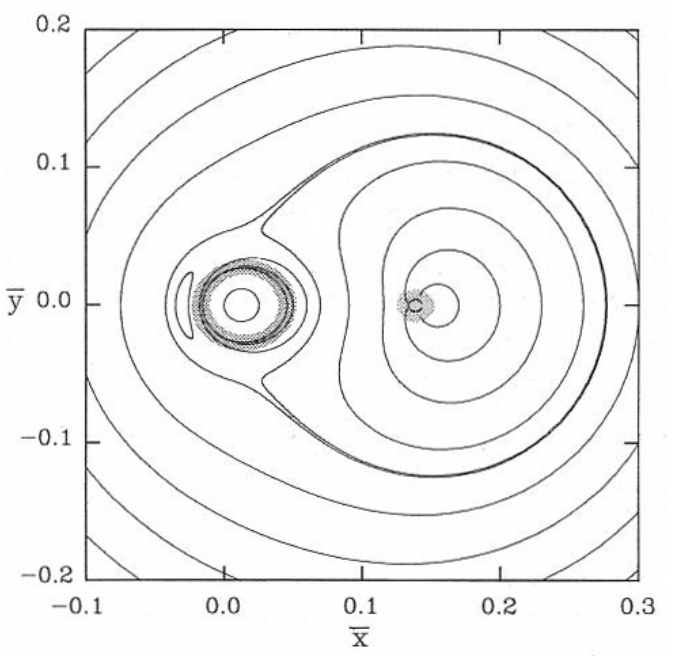
\includegraphics[scale=0.2]{img/p1.png}
        \caption{Траектории усредненной системы \\ при $\Delta H = -3.04 \cdot 10^{-6}$}
        \label{aver_fig}
    \end{minipage}%
    \begin{minipage}{0.5\textwidth}
        \centering
        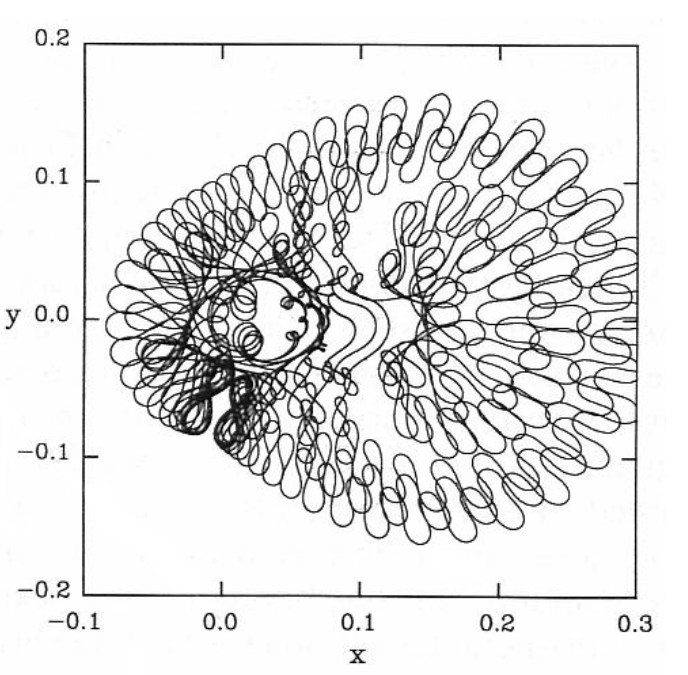
\includegraphics[scale=0.2]{img/p2.png}
        \caption{Траектории полной системы \\ при том же значении энергии}
        \label{real_fig}
    \end{minipage}
\end{figure}

Несмотря на свои преимущества, данный метод применим не для всех областей фазового пространства. В частности он перестает работать в том случае, когда период колебаний $\lambda$ становится сопоставим с периодами $\overline x$ и $\overline y$. Это происходит когда $\frac{d \lambda}{dt} = O(\mu)$ и, соответственно, сопоставимо с $\frac{dx}{dt}$ и $\frac{dx}{dt}$ в силу малости параметра $\mu$. Таким образом, для траектории системы при каждом прохождении в окрестности нулей функции $u(x,y)\sin \lambda - v(x,y) \cos \lambda$ изменяется значение (квази) адиабатического инварианта действия.

Как видно из рисунка \ref{real_fig}, траектория регулярно проходит через данную окрестность. По-видимому, этот факт является причиной расхождения теоретических и реальных границ эффекта.
%%%%%%%%%%%%%%%%%%%%%%%%%%%%%%%%%%%%%%%%%%%%%%%%%%%%%%%%%%%%%%%%%%%
